\chapter{Analysing Classes}
Python has two different kinds of classes, namely new and old style (or classic) classes that both support multiple inheritance. A new style class is one that contrary to an old style class inherits from the built-in class \inlinecode{object}. The two different kinds of classes vary among others in their method resolution order (MRO) \cite{pyref.typehierarchy}: old style classes resolves variables and attributes by a depth-first, left-to-right strategy, whereas new style classes use the more complex strategy C3 \cite{pyref.c3mro}, which is also known as the call-next-method from other multiple inheritance languages. Our motivation for supporting classes is the ability to analyse programs that use the magic method \inlinecode{\_\_getattr\_\_}. We have therefore only been working with classes that does not use inheritance. In this chapter we present our work towards handling class declarations, object creations, method invocations and attribute lookup on class instances for such classes.

%To start with consider the below example that illustrates the difference in MRO between new and old style classes.

%\begin{listing}[H]
%	\begin{minted}[linenos]{python}
%class A():
%	x = 'A'
%class B(A): pass
%class C(A):
%	x = 'C'
%class D(B, C): pass
%D().x # 'A'
%	\end{minted}
%	\caption{Multiple inheritance}\label{code:OldStyleMROExample}
%\end{listing}

%Since \inlinecode{D} extends \inlinecode{B} and \inlinecode{C}, which in turn extends the old style class \inlinecode{A}, \inlinecode{D} is itself an old style class. Therefore, evaluating \inlinecode{D().x} will result in \inlinecode{'A'}. If we instead had declared \inlinecode{A} as a new style class \inlinecode{class A(object): ...}, evaluating \inlinecode{D().x} would result in \inlinecode{'C'}.


\section{Class declarations}
In the CFG we have the following nodes related to class declarations: \textit{ClassDeclNode}, \textit{ClassEntryNode}, and \textit{ClassExitNode}. For \inlinecode{class C: <body>} we create a class declaration node in our CFG. Next, we create a class entry node which will become the successor of the class declaration node. Then, the inductively created CFG for \inlinecode{<body>} will be inserted after the class entry node, and finally, we create a class exit node and make it the successor of the exit node of the inductively created CFG for \inlinecode{<body>}.

\begin{listing}[H]
	\begin{center}
		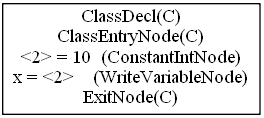
\includegraphics[width=0.5\textwidth]{images/class-decl-cfg.png}
	\end{center}
	\vspace{-10pt}
	\caption{The CFG generated by \inlinecode{class C: x = 10}.}
\end{listing}

The semantics of the three CFG nodes is the following:

\begin{itemize}
	\item The class declaration node, \textit{ClassDeclNode}, creates an empty class object on the abstract heap and sets the variable \inlinecode{C} to the newly created class object on the top object of the dynamic scope chain\footnote{Recall from \autoref{The Stack} that there may be more than one dynamic scope chain. In this case we write \inlinecode{C} to the top object of each of these scope chains.}. This makes the variable \inlinecode{C} available in the current scope.
	\item The class entry node, \textit{ClassEntryNode}, pushes the newly created class object onto the dynamic scope chain (for reasons we discuss in \autoref{section:Initializing empty class objects}).
	\item The class exit node, \textit{ClassExitNode}, reverts the scope chain to what it was before visiting the class entry node by popping the newly created class object from the dynamic scope chain.
\end{itemize}

The class declaration node and the class entry node could in principle be turned into a single node. We have chosen to have the two nodes in order to have a clear distinction between when the class object is created and when it is initialized in our analysis.


\subsection{Initializing empty class objects}
\label{section:Initializing empty class objects}
We add fields and methods to a newly created class object inbetween the class entry node and the class exit node. However, let us first describe how fields and methods can be added to classes in Python.

\begin{listing}[H]
	\begin{minted}[linenos]{python}
class C:
  x = 1
  def getX(self):
    return self.x

c = C() # C.x = 1, c.x = 1
C.x = 2 # C.x = 2, c.x = 2

def setX(self, x):
  self.x = x
C.setX = setX

c.setX(3) # C.x = 2, c.x = 3

c.setX = setX
c.setX(4) # TypeError: setX() takes exactly 2 arguments (1 given)
	\end{minted}
	\caption{Adding a field \inlinecode{x} and methods \inlinecode{getX} and \inlinecode{setX} to a class.}
	\label{code:FieldAndMethodOnClass}
\end{listing}

As \autoref{code:FieldAndMethodOnClass} illustrates, fields and methods can be created both at class declaration (lines 2-4) and later (lines 7, 11). It can also be seen that the fields and methods of the class are not copied to a newly created object at object creation (line 7).

The fields being added at class declaration are handled in the analysis by letting \textit{ClassEntryNode} push the class object onto the dynamic scope chain. For \inlinecode{x=1}, \inlinecode{x} is set to \inlinecode{1} as an attribute on the object on top of the dynamic scope chain (the class object).

However, since we cannot distinguish function declarations from method declarations in the CFG (both are declared using the \inlinecode{def} syntax), \inlinecode{getX} will appear as a function declaration. One problem is that the class instance is given implicitly as the first argument\footnote{As a consequence our lattice doesn't contain an explicit representation of the \inlinecode{this} keyword (unlike the lattice used by TAJS \cite{tajs}): we can simply treat \inlinecode{self} as a normal parameter to the function.} when calling methods (\autoref{code:FieldAndMethodOnClass}, line 13) but not functions (\autoref{code:FieldAndMethodOnClass}, line 16).

We handle the problem at function declaration in our analysis by checking whether the top object of the dynamic scope chain is a class object. In that case we wrap the function object in an unbound method object, which is merely a pointer to the function object; this ensures that the analysis is able to recognize when it should pass the class instance implicitly as the first argument. Otherwise we proceed as normal by handling the function declaration as explained in \autoref{Functions} about functions.

Another reason for wrapping the function object in an unbound method object is the following: it is not possible to write attributes on methods, but attributes on methods can be read in case the underlying function has the attribute.

This is illustrated by the following example:

\begin{listing}[H]
	\begin{minted}[linenos]{python}
class C: pass

def foo(self): pass
foo.attr = 42

C.foo = foo
C.foo.attr # 42
C.foo.attr = 0 # AttributeError: 'instancemethod' object has no attribute 'attr'
	\end{minted}
	\caption{It is not possible to set attributes on methods.}
\end{listing}

Fields and methods can also be added to a class after declaration time as was illustrated in \autoref{code:FieldAndMethodOnClass}. In our CFG this is represented by a \textit{WriteAttributeNode}. As for write variable nodes we check whether the object being written to is a class object. If it is, and the value being written is a function, we wrap the function object in an unbound method object.

An important thing with regards to scoping which is pointed out in \cite{lamdapy} (page 10) is that variables declared inside a class are \textit{not} available as variables inside the methods of the class. For instance, accessing \inlinecode{x} inside the method \inlinecode{getX} in (\autoref{code:FieldAndMethodOnClass}) would result in a \inlinecode{NameError}. It should be accessed as \inlinecode{C.x} or \inlinecode{self.x}.


\section{Object creations}
\label{section: Object creations}
As we already discussed the analysis cannot necessarily distinguish a function call from an object creation. At each \textit{CallNode} in our CFG we therefore investigate which kind of object on the abstract heap is being called. If it is a class object that is being called, we create a new instance object on the abstract heap, representing the newly created instance. In particular, we do not modify the call graph as we do for function calls unless the magic method \inlinecode{\_\_init\_\_} has been implemented (see \autoref{section:Constructor calls}, Constructor calls).

\begin{listing}[H]
	\begin{minted}[linenos]{python}
if (trickyComputation()):
  class C: pass
else:
  def C(): return 42
x = C()
	\end{minted}
	\caption{It is not possible to statically determine if \inlinecode{C} is a class or function.}
	\label{code:BothNewOldClassAndFunction}
\end{listing}

In \autoref{code:BothNewOldClassAndFunction} it is not possible to tell whether \inlinecode{C} after the \inlinecode{if} statement is pointing to the class in line 2, or the function in line 4. Therefore, our analysis will conclude that \inlinecode{x} is either a pointer to a class instance, or the integer 42. This is seen in the figure below generated by our type analysis, which is the output of the heap at the exit node of the CFG for this particular example.

\begin{listing}[H]
	\begin{center}
		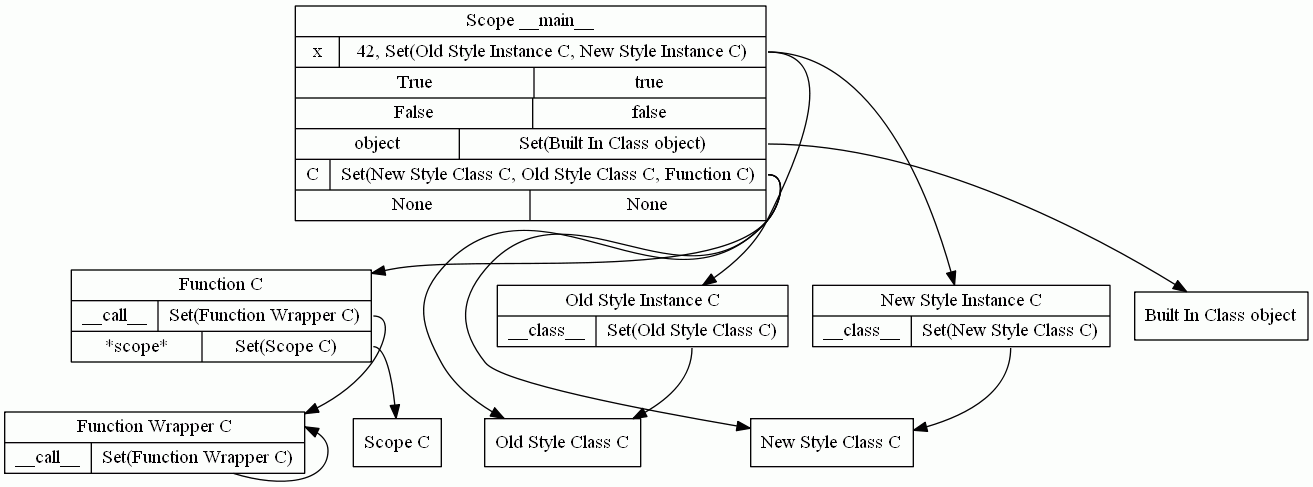
\includegraphics[width=1\textwidth]{images/BothNewOldClassAndFunction.png}
	\end{center}
	\vspace{-10pt}
	\caption{Part of the heap generated by our analysis tool.}
	\label{fig:BothNewOldClassAndFunction}
\end{listing}


\subsection{Constructor calls}
\label{section:Constructor calls}
The magic method \inlinecode{\_\_init\_\_} can be set on a class in order to supply a constructor.

\begin{listing}[H]
	\begin{minted}[linenos]{python}
class C:
  def __init__(self, x):
    self.x = x
c = C(42)
c.x # 42
	\end{minted}
	\caption{The magic method \inlinecode{\_\_init\_\_} can be implemented to supply a constructor.}
	\label{code:InitConstructorClass}
\end{listing}

This introduces a minor issue that arises from the fact that the analysis cannot distinguish object creations from function invocations at first sight. What happens at line 4 in \autoref{code:InitConstructorClass} above is the following:

\begin{enumerate}
	\item A class instance object is created on the abstract heap because of the call to a class object.
	\item A value pointing to this newly created instance object is stored in the special return register on the abstract stack.
	\item The call graph is updated with call edges from the call node to the entry node of \inlinecode{\_\_init\_\_}, and from the exit node of \inlinecode{\_\_init\_\_} to the after call node.
	\item As a result of (3) the return value of \inlinecode{\_\_init\_\_} is stored in the special return register. Note that the return value of \inlinecode{\_\_init\_\_} must be the built-in constant \inlinecode{None}; otherwise a type error results (for this example our analysis will insert an implicit return \inlinecode{None} node in the CFG).
	\item The after call node will now read the value from the special return register on the abstract stack and store it; in this case as the attribute \inlinecode{x} of \inlinecode{c}.
\end{enumerate}

For this approach the best we can do is to take the least upper bound when we write to the special return register. As a consequence the variable \inlinecode{c} from \autoref{code:InitConstructorClass} will map to an abstract value corresponding to either \inlinecode{None} or an instance object. This would mean that the analysis should report a type error in line 5, because an attribute is possibly being dereferenced on a non-object, \inlinecode{None}.

We solve this issue by introducing a new special constructor return register, where we store newly created class instances, together with a new kind of call edge in the call graph; constructor call edges.

The idea is the following: instead of updating the call graph with call edges in (3) we update it with constructor call edges. This means that we can recognize returns from \inlinecode{\_\_init\_\_} functions, check that they are indeed \inlinecode{\_\_None\_\_} and then ignore it.

Specifically, our implementation has a special join operation for after call nodes\footnote{for all other nodes the join operation just takes the least upper bound of the solutions of its predecessors.}. The join operation for after call nodes is the usual join operation, except that solutions coming from constructor call edges have their special return register (containing \inlinecode{\_\_None\_\_}) emptied. As a consequence, our analysis can just take the least upper bound of the values in the special return and the special constructor return register, and store it appropriately e.g. as the attribute \inlinecode{x} of \inlinecode{c}.


\section{Built-in constants, functions and classes}
To support some of the built-in constants, functions and classes that are available in Python we have given abstract implementations of them in a file \inlinecode{\_\_builtin\_\_.py}, which is imported every time the analysis runs. For instance we initialize the built-in constant \inlinecode{True} as follows: \inlinecode{True = \_\_BooleanLattice\_Concrete\_TRUE\_\_}. Here, \inlinecode{\_\_BooleanLattice\_Concrete\_TRUE\_\_} is a special name recognized by our type analyser.

\begin{listing}[H]
	\begin{minted}[linenos]{python}
def raw_input():
  return __StringLattice_Abstract__
	\end{minted}
	\caption{The implementation of \inlinecode{raw\_input}, that takes general input from users, in \inlinecode{\_\_builtin\_\_.py}.}
\end{listing}

The idea of using the target language to implement some of the built-in structures is common in static analysis and can be seen in both TAJS \cite{tajs} and Lambda Py \cite{lambdapy} (section 6.2), even though these projects have different approaches to static analysis.


%\section{A note on handling both new and old style classes}
%As mentioned we only handle classes that does not use inheritance in our analysis. If we were to handle both kinds of classes it would not be enough to only create one class object on the abstract heap for each class declaration.

%\begin{itemize}
%	\item If \inlinecode{C} is definitely a new style class a new style class object is created on the heap, likewise for old style classes.
%	\item Otherwise, both a new style class object and an old style class object is created on the heap.
%\end{itemize}

%For the example in \autoref{code:OldStyleMROExample} our analysis will only create an old style class object on the heap, however for the below example we generate two objects.

%\begin{listing}[H]
%	\begin{minted}[linenos]{python}
%if (...):
%  class B(): pass
%else:
%  class B(object): pass
%class C(B): pass
%	\end{minted}
%	\caption{An example where we can't conclude that \inlinecode{C} is definitely a new style class or definitely an old style class.}\label{code:NotDefinatelyNewOldStyleClass}
%\end{listing}

%We conclude that a class is definitely a new style class if the following holds:

%\begin{enumerate}
%	\item The built-in class \inlinecode{object} has not been overwritten.
%\end{enumerate}

%Of course it would still be possible to conclude that \inlinecode{class C(O): ...} is a new style class if the variable \inlinecode{O} has been set to \inlinecode{object} before overwriting \inlinecode{object} like in the below example.

%\begin{listing}[H]
%	\begin{minted}[linenos]{python}
%O = object
% object = 42
% class C(O): pass
% 	\end{minted}
% 	\caption{The class \inlinecode{C} here is easily seen to be a new style class.}\label{code:ClassOverwrittenObject}
% \end{listing}

% However, our implementation does not at the moment check this because of the limited time of our project, and the fact that programmers should really not overwrite the built-in \inlinecode{object}. Note that our implementation does conclude that \inlinecode{class C(O): ...} is a new style class if line 2 in the example had been skipped.

% If \inlinecode{object} has not been overwritten, we check that:

% \begin{enumerate}
% \setcounter{enumi}{1}
% 	\item All the base classes \inlinecode{B1}, ..., \inlinecode{Bn} are either the built-in object or definitely a new style class.
% \end{enumerate}

% Recall that the base classes \inlinecode{B1}, ..., \inlinecode{Bn} are just variable names. If \inlinecode{Bi} is the variable \inlinecode{object}, we can conclude that it is the built-in object since we from (1) have that the built-in \inlinecode{object} has not been overwritten. If \inlinecode{Bi} is not \inlinecode{object} we look up the variable on the scope chain, and make sure its value is only a pointer to a new style class object on the heap, or the built-in class \inlinecode{object}. If it is for instance a pointer to either a new style class object or an old style class object (see for instance \autoref{code:NotDefinatelyNewOldStyleClass}), we conclude that the class \inlinecode{C} it is not definitely a new style class object.

% In the same way we conclude that a class is definitely an old style class.